\documentclass[utf8]{gradu3}

\usepackage{graphicx}
\usepackage{amsmath}
\usepackage{booktabs}
\usepackage[backend=biber]{biblatex}
\usepackage[dvipsnames]{xcolor}

% HUOM! Tämän tulee olla viimeinen \usepackage koko dokumentissa!
\usepackage[bookmarksopen,bookmarksnumbered,linktocpage]{hyperref}

\addbibresource{gradubibtex.bib}

\begin{document}

\title{Puheen ongelmista kärsiville tarkoitetun kommunikointisovelluksen toteuttaminen Ionic-kehyksellä}
\translatedtitle{Puheen ongelmista kärsiville tarkoitetun kommunikointisovelluksen toteuttaminen Ionic-kehyksellä}
\studyline{Ohjelmistotekniikka}
\avainsanat{%
  Ionic,
  AAC,
  WWW-sovellukset,
  käytettävyys
}
\keywords{%
  Ionic,
  AAC,
  web applications,
  usability
}
\tiivistelma{%
  Tutkielman tiivistelmä on tyypillisesti lyhyt esitys, jossa kerrotaan tutkielman taustoista, tavoitteesta, tutkimusmenetelmistä, saavutetuista tuloksista, tulosten tulkinnasta ja johtopäätöksistä. Tiivistelmän tulee olla niin lyhyt, että se, englanninkielinen abstrakti ja muut metatiedot mahtuvat kaikki samalle sivulle.
}
\abstract{%
  Tiivistelmä englanniksi.
}

\author{Roope Kivioja}
\contactinformation{\texttt{roope.kivioja@gmail.com}}

\supervisor{Jukka-Pekka Santanen}
\supervisor{Jonne Itkonen}

\maketitle

\begin{thetermlist}
\item[Ionic] Ohjelmistokehys.
\end{thetermlist}

\mainmatter

\chapter{Johdanto}
\colorbox{YellowGreen}{// Ohjepituus 5 sivua.}

\colorbox{YellowGreen}{// TODO: Tähän tulee johdanto.}

\chapter{Kommunikointisovelluksen rakentamiseen tarvittavia taustatietoja ja menetelmiä}
\colorbox{YellowGreen}{// Ohjepituus 10-15 sivua.}

\colorbox{YellowGreen}{// TODO: Lyhyt siltaava kappale johdannosta teoriakappaleeseen}

\colorbox{YellowGreen}{// TODO: kirjoita omaksi kappaleeksi:}

- Taustat, tarpeet ja tavoitteet:

- progressiivisten WWW-sovellusten tutkiminen

- progressiivisten WWW-sovellusten sopiminen avusteisen kommunikaation mobiilisovelluksien tuottamiseen

-> tavoite: Ionic-kehyksen toiminnan tutkiminen

-> tavoite: Ionic-kehyksen avulla tehdyn avusteisen kommunikaation sovelluksen vertaaminen ohjelmistoteknisiin ja käytettävyyspohjaisiin suosituksiin kehittäjän näkökulmasta

-> tavoite: Ionic-kehyksen avulla tehdyn avusteisen kommunikaation sovelluksen soveltuminen autistien kätettävyystarpeisiin suosituksien pohjalta

\section{Avusteinen kommunikaatio}

On olemassa useita eri sairauksia ja kehityshäiriöitä, joiden johdosta henkilön kyky muodostaa puhetta voi hetkellisesti tai pysyvästi heikentyä. Puheen muodostamisen ongelmista kärsivä henkilö saattaa joutua turvautumaan arkipäivän kommunikaatiossa erilaisiin apuvälineisiin kommunikoidakseen muiden ihmisten kanssa. Yleisesti näitä viestintämenetelmiä kuvaamaan tarkoitettu termi on \textbf{puhetta tukeva ja korvaava kommunikaatio} (engl. \textit{Augmentative and Alternative Communication, lyh. AAC}).

Puhetta tukeva ja korvaava kommunikaatio voidaan jakaa kahtia: avustamattomaan ja avusteiseen. \textbf{Avustamattomalla puhetta tukevalla ja korvaavalla kommunikaatiolla} tarkoitetaan kommunikaatiota, jossa ei tarvita apuvälineitä. Viittomakieli on yksi esimerkki avustamattomasta puhetta tukevasta ja korvaavasta kommunikaatiosta, mutta myös ihmisen elekieltä voidaan pitää avustamattomana puhetta tukevana ja korvaavana kommunikaationa. 

\textbf{Avustettu puhetta tukevaa ja korvaava kommunikaatio} tarkoittaa puolestaan kommunikaatiota, jossa käytetään jotain apuvälinettä. Apuvälineenä voi olla esimerkiksi valokuvia, kommunikaatiotaulu tai elektroninen laite. Tämän perusteella avustettu puhetta tukevaa ja korvaava kommunikaatio voidaan jakaa vielä eteenpäin kahdeksi ryhmäksi: matalan teknologian ja korkean teknologian puhetta tukevaan ja korvaavaan kommunikaatioon. Käyttäjä ei välttämättä käytä vain yhtä edellä mainituista tyypeistä. \parencite[]{AAC-conditional-use}

Puhetta tukevaa ja korvaavaa kommunikaatiota voidaan tarjota puheen muodostamisen ongelmista kärsiville myös tietoteknisten sovellusten avulla, joiden kautta käyttäjä kirjoittaa joko suoraan tekstiä tai kommunikoi valitsemalla symboleja. Esimerkiksi autistisilla käyttäjillä on tyypillisesti hyvin henkilö- ja yksityiskohtaisia tarpeita puhetta tukevalle ja korvaavalle kommunikaatiolle, joten tietoteknisten sovellusten suhteellisen helppo muokattavuus puoltaa niiden käyttöä perinteisempien puhetta ja kommunikointia korvaavien apuvälineiden sijaan.

Puhetta tukevat ja korvaavat kommunikointisovellukset käyttävät yleisimmin symboleja. Autisteille tyypillistä on vahva visuaalis-avaruudellinen hahmotuskyky, joten tutkimuksen mukaan piirroksiin ja valokuviin liitetyt merkitykset ovat tälle ryhmälle luontevin tapa kommunikoida. Vaughnin ja Hornerin tutkimuksessa  \parencite[]{concrete-versus-verbal} Karl-nimisen autistisen koehenkilön haastava käytös ja aggressio vähenivät kun pelkästään verbaalisesti annettujen ruokavaihtoehtojen rinnalle tuotiin kuvat ruoka-annoksista. Symbolipohjaiselle puhetta tukevalle ja korvaavalle kommunikaatiolle on siis sekä tutkimuspohjaista näyttöä, että käytännön kokemuksiin perustuvaa kannustetta.

Puhetta tukevaan ja korvaavaan kommunikointisovellukseen voidaan liittää myös symboleita lukeva ääniominaisuus. Ääniominaisuus mahdollistaa kommunikoinnin näköyhteyden ulkopuolelle, vähentää symbolien tulkitsijan läsnäolon pakollisuutta ja helpottaa pidempien viestien rakentamista puhetta tukevassa ja korvaavassa kommunikointisovelluksessa. \parencite[]{AAC-interventions}

\colorbox{YellowGreen}{// TODO: ankkuroi edellinen kappale paremmin tekstiin}

Esimerkiksi ääniominaisuuden lisäämisellä avustetusta puhetta tukevasta ja korvaavasta kommunikaatiosta voidaan tehdä \textbf{monimodaalista}. Monimodaalisuus tarkoittaa usean eri kommunikaatiotavan kautta tapahtuvaa kommunikaatiota. Monimodaalinen kommunikaatio voi tapahtua eri tapojen kautta yhtäaikaisesti tai peräkkäin. Puhetta tukevasta ja korvaavasta kommunikaatiosta kannattaa tehdä monimodaalista useista eri syistä. Ensinnäkin, suurin osa kaikesta kommunikaatiosta on monimodaalista: toiselle ihmiselle puhuttaessa on tavallista selkeyttää sanomaa ilmein ja elein. Toiseksi, puhetta tukevaa ja korvaavaa kommunikaatiota käyttävä henkilön tarvitsee useasti kommunikoida muiden puhetta tukevaa ja korvaavaa kommunikaatiota käyttävien henkilöiden kanssa, jolloin vaihtoehdoista on hyötyä. Kolmas merkittävä syy on se, että eri puhetta tukevissa ja korvaavissa kommuunikaatiotavoissa on vahvuuksia ja heikkouksia, joten eri kommunikaatiotapoja sekoittamalla voidaan korvata yksittäisen kommunikaatiotavan heikkouksia. \parencite[]{AAC-conditional-use}

\colorbox{YellowGreen}{// TODO: mitä ongelmia} 

\section{Progressiiviset WWW-sovellukset}

\textbf{Progressiiviset sovellukset} (engl. \textit{Progressive web applications, lyh. PWAs}) ovat selaimessa ajettavia WWW-sovelluksia, joiden ulkoasu määrittyy alustakohtaisesti niin, että niiden ulkoasu on mahdollisimman yhdenmukainen laitteen natiivien sovellusten kanssa. Selainpohjaisuuden takia progressiiviset sovellukset pystyvät käyttämään tarjolla olevia sovellusympäristön resursseja joustavasti sen sijaan, että ne itse määrittäisivät vaatimukset. Termi on verrattain tuore ja vakiintumaton, sillä esimerkiksi Ionic-kehyksen dokumentaatiossa käytetään myös termiä \textbf{hybridisovellus} (engl. \textit{hybrid application}).

Progressiivisten sovellusten ilmeisin hyöty on alustariippumattomuus. Samaa sovellusta voidaan käyttää kaikissa ympäristöissä, jotka tukevat WWW-selaimia. Eri versioita samasta sovelluksesta ei tarvitse kehittää ja ylläpitää erikseen, joten progressiivisten sovellusten avulla voidaan säästää kalliita työresursseja. Hyvä esimerkki progressiivisten sovellusten käyttöä tukevasta markkinatilanteesta on nykyisten älytelevisioiden kirjava tarjonta: valmistajien omien käyttöjärjestelmien lisäksi muunmuassa Apple, Amazon ja Roku kehittävät televisioon liitettäviä laitteita, joiden avulla käyttäjä voi ajaa erilaisia sovelluksia. Näiden kaikkien laitteiden tukeminen olisi hyvin vaikeaa perinteisten sovellusten avulla. \parencite[]{frankston-pwa}

Tällä hetkellä erityisesti Google panostaa progressiivisten sovellusten kehittämiseen Chrome-selaimen kehitysympäristön yhteydessä. Googlen \parencite[]{google-pwa-marketing} mukaan progressiiviset sovellukset tarjoavat perinteisiin WWW-sovelluksiin verrattuna enemmän luotettavuutta, käytettävyyttä ja monipuolisempaa sisältöä. Yrityksen mukaan luotettavuus paranee, sillä progressiiviset sovellukset pystyvät tarjoamaan sisältöä myös ilman verkkoyhteyttä. Google myös väittää, että progressiivisten sovellusten kohdalla käytettävyyttä parantaa nopeammin käyttäjän komentoihin vastaava käyttöliittymä ja sovellusmaisuus puolestaan parantaa käyttäjän immersiota.

Googlen Chrome-selain on rakennettu avoimen lähdekoodin Chromium-selaimen päälle. Yksi merkittävimmistä Chromium-selaimeen pohjautuvista progressiivisten WWW-sovellusten kehitykseen tarkoitetuista kehyksistä on Electron. Electron on Microsoftin nykyisin omistaman GitHubin kehittämä ja ylläpitämä. Esimerkkejä Electron-sovelluksista ovat Discord, Slack ja Visual Studio Code. On mahdollista, että Microsoftin päätös muuttaa Edge-selain Chromium-pohjaiseksi johtui ainakin osittain progressiivisten WWW-sovellusten vaatimista ominaisuuksista kuten tehokkaammasta muistinhallinnasta.

Twitter, AliExpress ja Lancôme ottivat vuonna 2017 käyttöön progressiiviset sovellukset ja julkaistut tulokset ovat olleet positiivisia. Twitter onnistui uuden progressiivisen sovelluksensa ansiosta lisäämään sivupäivityksiä 65\% per sessio, lisäämään lähetettyjen Twitter-viestien määrää 75\% ja vähentämään käytön lopettamista 20\%. Lisäksi uusi sovellus käytti vähemmän kuin 3\% natiivin sovelluksen vaatimasta muistitilasta ja vähensi datan käyttöä 70\%. Datan käytön määrän vähentyminen on erityisen merkittävää, koska Twitter arvioi, että vuonna 2017 45\% sen sisällöstä ladattiin 2G-verkon läpi. \parencite[]{beginners-guide-pwa}

AliExpress ja Lancôme ovat molemmat verkkokauppoja, joilla on ollut ongelmia mobiiliverkkokauppojensa tehokkuuden kanssa. Progressiiviseen sovellukseen siirtymällä AliExpress lisäsi uusien asiakkaiden myyntitapahtumien määrää 104\%:lla ja Lancôme 17\%:lla. Lisäksi AliExpress tuplasi sivunlatausten määrän sekä kasvatti sessioiden pituutta 74\%:lla. Lancôme puolestaan onnistui lisäämään iOS-sessioiden määrää 53\%:lla. \parencite[]{beginners-guide-pwa} Edellä mainitut tulokset eivät kuitenkaan ole suoraan yleistettävissä yleisemmin progressiivisten sovellusten vaikutuksiin, sillä niiden otoskoko on erittäin pieni.

Progressiivisten sovellusten käyttö ei kuitenkaan ole ongelmatonta. Ensinnäkin, koska progressiivisten WWW-sovellusten hyödyntämät teknologiset kehitysaskeleet ja niiden käyttöön kannustavat taloudelliset tekijät ovat verrattain tuoreita, vaaditaan kehittäjiltä paljon uusien asioiden opettelua sekä vakiintumattomien työkalujen sekä kehysten käyttämistä kehitystyössä. Toinen merkittävä haaste voi olla tiedon tallentaminen, sillä selaimen toimintaan pohjautuvalle sovellukselle ei ole varattu tietoturvan takia samoja oikeuksia kuin natiiveille sovelluksille. Kolmas ongelma voi tulla eteen käytettävyydessä, sillä selaimessa toimivan sovelluksen vaatimat resurssit saattavat hidastaa sovelluksen toimintaa. \parencite[]{pwa-design-challenges}

Myös progressiivisten sovellusten muistinkäyttöä on kritisoitu. Progressiiviset sovellukset vaativat perinteisiä sovelluksia enemmän muistia, koska niitä ajetaan selaimen päällä. On vaikea arvioida kuinka suuri osa muistinkäytöstä johtuu sovelluksen toteutuksesta ja kuinka suuri osa itse ohjelmistokehyksestä, mutta hyvin yksinkertaisissakin testeissä on saatu tuloksia, jotka viittaavat moninkertaiseen muistinkäyttöön natiiveihin sovelluksiin verrattuna \parencite[]{electron-memory-usage}.

\colorbox{YellowGreen}{// - TODO: tähän omaa kriittistä pohdintaa}

Progressiiviset WWW-sovellukset sopivat siis parhaiten tilanteisiin, joissa vähän muistia vaativan sovelluksen halutaan tukevan useita eri alustoja, mutta joissa tavallinen WWW-sivu ei riitä. Avusteisen kommunikaation sovelluksien vaatimukset osuvat hyvin yhteen progressiivisten WWW-sovellusten vaatimusten kanssa, sillä kuvakorttien näyttäminen ei ole muisti-intensiivistä, mutta toisaalta taas avusteisen kommunikaation sovellusten halutaan olevan helposti muovattavissa henkilökohtaisiin tarpeisiin sopiviksi sekä toimivan useilla eri alustoilla.

\section{Ionic-ohjelmistokehyksen rakenne ja ominaisuudet}

Ionic on yksi suosituimpia progressiivisten sovellusten tuottamiseen suunnitelluista ohjelmistokehyksistä. Electronin ollessa kiinteille päätteille suunnattu kehys, Ionic keskittyy mobiililaitteiden vaatimuksiin. Ionic on avointa lähdekoodia ja hyödyntää Apache Cordova -ympäristöä sekä Angular-ohjelmistokehystä. Ionic on MIT-lisenssin alainen ja täten avointa lähdekoodia. Angular-ohjelmistokehys perustuu TypeScript-ohjelmointikieleen. Ionicin perusrakenne on kuvattuna kaaviossa \ref{fig:ionic-structure}. Kehyksenä Ionicin pääpaino on tarjota kehittäjälle oikealta näyttävä ja visuaalisesti toimiva sovellus. Sen ei ole tarkoitus korvata tyypillisiä JavaScript-kirjastoja vaan se toimii niiden tukena. \parencite[]{ionic-documentation}

Ionicia ylläpitää ja kehittää Ben Sperryn ja Max Lynch perustama samanniminen yritys. Avoimen lähdekoodin projektina Ionic-kehyksen kehitykseen ja ylläpitoon pääsee osallistumaan GitHub-sivuston välityksellä kuka tahansa. Ionicin viimeisin pääversio on 4.0.0. Viime aikoina Ionicin kehitystyössä painoarvoa on annettu erityisesti Ionic-kehyksen ja Angularin välisten riippuvuuksien vähentämiseen, jotta Ionicia voitaisiin käyttää muiden kehyksien kuten Reactin ja Vue.js:n yhteydessä.

\begin{figure}[h]\centering
  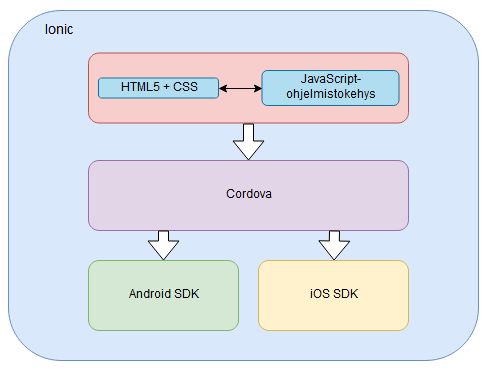
\includegraphics[height=9cm,keepaspectratio]{ionic-structure}
  \caption[Ionic-sovelluksen perusrakenne]
  {Ionic-sovelluksen perusrakenne.}
  \label{fig:ionic-structure}
\end{figure}

Ionic koostuu komponenteista. Ionicin komponentit ovat uudelleenkäytettäviä käyttöliittymäelementtejä, jotka toimivat sovelluksen käyttöliittymän rakennusosina. Niiden avulla sovellus näyttää yhtenäiseltä ja käyttöliittymän kehitystyö nopeutuu. Komponentit koostuvat HTML:stä, CSS:stä ja JavaScriptistä. Esimerkkejä tällaisista komponenteista ovat muunmuassa painikkeet, välilehdet ja erilaiset listat. Ionicin toteutuksessa on pyritty tukemaan näiden komponenttien mahdollisimman joustavaa kustomointia \parencite[]{ionic-documentation}.

Ionicin ulkoasu perustuu teemoihin. Myös teemat lisäävät sovelluksen ulkoasun yhtenäisyyttä. Teemat myös mukautuvat eri alustojen ulkoasustandardien mukaisiksi kehittäjän niin halutessa. Esimerkiksi Android- ja iOS-mobiilikäyttöjärjestelmille suunnattujen sovellusten ulkoasu poikkeaa toisistaan, jos käytetään Ionicin oletusteemoja. Teemojen käyttäminen parantaa sovelluksen käytettävyyttä tekemällä sen ulkoasusta ennustettavamman ja tutumman loppukäyttäjälle. Ionicin oletusteemat noudattavat Applen iOS-designperiaatteita sekä Googlen Material Design -määrityksiä.

\subsection{Apache Cordova}

Apache Cordova (aikaisemmin PhoneGap) on alunperin Nitobin kehittämä sovelluskehitysympäristö mobiililaitteille. Adobe osti Nitobin vuonna 2011 ja myöhemmin uudelleenjulkaisi Apache Cordovan avoimena lähdekoodina. Apache Cordova toimii WWW-sovelluskehyksien ja natiivien sovelluskehyksien välisenä linkityskerroksena \parencite[]{ionic-framework-hybrid}. Apache Cordovan avulla Ionic ja muut Apache Cordovan päälle rakennetut ohjelmistokehykset voivat toimia syvemmällä tasolla kuin tyypillinen WWW-sovellus, sillä niille tarjoutuu rajapinta suoraan natiiveihin sovelluskehyksiin. Näin progressiivisille WWW-sovelluksille tarjoutuu mahdollisuus käyttää muunmuassa mobiililaitteen kameraa ja GPS-paikannusta.

\subsection{Angular}

Angular on Googlen Angular Teamin ylläpitämä TypeScript-pohjainen käyttöliittymäkehys. Se on jatkoa aiemmin ilmestyneelle AngularJS-kehykselle. Alkuperäinen AngularJS-kehys julkaistiin vuonna 2010, ja se oli ensimmäinen suosittu ohjelmistokehys dynaamisten HTML-sivujen tuottamiseen mahdollistaen tehokkaamman yhden sivun WWW-sovellusten rakentamisen. Angular julkaistiin vuonna 2016, ja se on kokonaan uudelleenohjelmoitu versio AngularJS:stä.

AngularJS perustuu MVC-arkkitehtuuriin, kun taas uudempi Angular on komponenttipohjainen. Komponenttipohjainen arkkitehtuuri pyrkii tarjoamaan paremman uudelleenkäytettävyyden, luettavuuden, testattavuuden ja ylläpidettävyyden. Ohjelma jaetaan itsenäisiin komponentteihin, joita voidaan käyttää useasti ja niiden itsenäisyys helpottaa yksikkötestaamista. Itsenäiset komponentit ovat huomattavasti helpommin ymmärrettävissä ja niiden korvaaminen on joustavampaa, mikä parantaa ylläpidettävyyttä. \parencite[]{good-and-bad-angular} 

Angularin komponenttipohjainen rakenne perustuu kolmeen hiljattain ilmestyneeseen teknologiaan: \textbf{Web-komponentteihin} (\textit{engl. Web Components}), JavaScriptin ES2015-standardiin ja TypeScript-ohjelmointikieleen.

Web-komponentit on laaja-alainen termi, jolla tarkoitetaan neljää WWW-selaimissa yleistyvää standardia: \textbf{kustomoitavat elementit} (\textit{engl. custom elements}), \textbf{varjo-DOM} (\textit{engl. shadow DOM}), \textbf{mallit} (\textit{engl. templates}) ja \textbf{HTML-tuonti} (\textit{engl. HTML imports}). Kustomoitavat HTML-elementit ovat HTML-standardielementtien ulkopuolisia elementtejä, joita voidaan käyttää standardielementtien seassa. Kustomoitava HTML-elementti irroittaa komponentin sivun muista osista, joten se mahdollistaa komponentin eristämisen. Varjo-DOM on piiloitettu osa sivua, jolla on oma eristetty ympäristö skripteille, CSS-tyylitiedostoille ja HTML-elementeille. Varjo-DOM:n elementit ja tyylit eivät vaikuta varjo-DOM:n ulkopuolisiin alueisiin ja vastavuoroisesti muut sivun elementit ja tyylit eivät vaikuta varjo-DOM:n alaisiin osiin. Komponentti voi täten käyttää tätä eristettyä aluetta renderöintiin. Mallit ovat HTML-palasia, jotka eivät lataudu välittömästi HTML-sivun auetessa vaan ne voidaan aktivoida JavaScriptillä myöhemmin. Malleista on useita toteutuksia eri kehyksissä, mutta Web-komponentit standardisoivat mallien rakentamisen ja tarjoavat suoran tuen niiden hyödyntämiselle selaimessa. Malleja käyttämällä varjo-DOMiin piilotetusta sisällöstä voidaan tehdä dynaamista. Viimeinen web-komponenttien osa on HTML-tuonti. HTML-tuonnin avulla HTML-, CSS- ja JavaScript-tiedostoja voidaan ladata yhtenäisinä osina. Angular ei käytä HTML-tuontia vaan se käyttää JavaScriptin moduulilatausta. \parencite[]{angular-6-by-example}

\subsection{TypeScript}

TypeScript on avoimen lähdekoodin ohjelmointikieli, jota ylläpitää Microsoft. TypeScript kääntyy suoritusvaiheessa JavaScriptiksi, ja se on tarkoitettu tukemaan JavaScript-ohjelmien kehitystä parantelemalla JavaScriptin ominaisuuksia. TypeScript sisältää ES 2015 -standardin mukaiset ominaisuudet sekä lisäksi se tarjoaa ohjelmoijan käyttöön tyypit ja koristelijat. Angular-ohjelmointikehyksen ohjelmointiin käytetään TypeScript-ohjelmointikieltä.

TypeScriptin on tarkoitus tarjota Microsoftin .NET-ympäristöön tottuneille ohjelmoijille oliolähtöisempi lähestymistapa JavaScript-kehitykseen \parencite[]{maharry-typescript}. JavaScript on suosittu ohjelmointikieli, mutta varsinkin ohjelmiston lähdekoodin määrän kasvaessa sen heikkoudet alkavat tulla esiin. TypeScript pyrkii puuttumaan näihin ongelmiin tarjoamalla ohjelmoijalle moduulijärjestelmän, luokat, rajapinnat ja staattisen tyypityksen \parencite[]{understanding-typescript}.

Ohjelmointikielen modulaarisuudella tarkoitetaan sitä, että muuttujat, funktiot, luokat ja muut vastaavat ohjelmointikielen perusrakenteet ovat olemassa vain moduulien sisällä, ellei niitä erikseen esitellä muille moduuleille \parencite[]{typescript-modules}. Tämä vähentää ohjelman eri osien välistä riippuvuutta toisistaan, mikä helpottaa muutosten tekemistä ohjelmistoon.

Perinteisesti JavaScript on käyttänyt uudestikäytettävien komponenttien rakentamiseen funktioita ja prototyyppipohjaista perintää. Iso osa nykyohjelmoijista ei kuitenkaan ole tottunut käyttämään edellä mainittuja keinoja, vaan nykyisin suosituin lähestymistapa uudelleenkäytettävyyteen on luokkien käyttäminen. \parencite[]{typescript-classes}

Uudelleenkäytettävyyden lisäksi TypeScriptin luokkien avulla saadaan JavaScriptiin verrattuna helpommin aikaan modulaarisia komponentteja, joita on helpompi ylläpitää ja skaalata. Virheiden löytämistä helpottaa se, että luokkien avulla ohjelmakoodin rajoista saadaan selkeämpiä. Skaalautuvuutta varten täytyy monesti pystyä korvaamaan vanhoja komponentteja uusilla ja luokkia käyttämällä myös tämä on helpompaa.

\textbf{Rajapintoja} käytetään kuvaamaan luokkien ominaisuuksia. TypeScriptissä rajapintoja käytetään tyyppien nimeämiseen ja niiden avulla voidaan tehdä olioiden välisiä sopimuksia ohjelmoijan itse laatiman ohjelmistokoodin sisällä sekä myös ohjelmoijan oman ohjelmistokoodin ja muiden tuottamien kirjastojen välillä. \parencite[]{typescript-interfaces} Esimerkiksi Swagger-niminen työkalu generoi .NET-palvelinkoodista valmiita rajapintoja, joita TypeScript-pohjaisen WWW-sovelluksen on helpompi käyttää. Rajapinnat ovat luonnollinen jatke luokille. Niiden avulla luokan toteutus voidaan eroittaa sen ulkopuolelle näkyvistä osista ja jakaa luokkia ryhmiin. Kuten luokkienkin kohdalla, rajapintojen käyttäminen voi parantaa ohjelman ylläpidettävyyttä, skaalautuvuutta ja osien uudelleenkäytettävyyttä.

TypeScript on dynaamisesti tyypitetty kieli samoin kuin JavaScript, mutta se noudattaa \textbf{ankkatyypitystä} (engl. duck typing). Ankkatyypitys tarkoittaa sitä, että luokan käyttömahdollisuudet eivät määrity sen tyypin perusteella vaan luokkaa voidaan käyttää sen ominaisuuksien ja metodien perusteella.

JavaScriptistä poiketen TypeScriptin tyypitys on myös vahvaa. Vahvalla tyypityksellä tarkoitetaan sitä, että tyyppien täytyy olla operaatioissa toisiaan vastaavia. Vahvan tyypityksen avulla ohjelmoijan on helpompi nähdä suoraan, että ohjelman tieto on oikean tyyppistä sitä käsitellessä. Iso osa tyyppivirheistä jää tällöin kiinni jo ennen kääntämistä kun taas JavaScriptilla ohjelmoidun ohjelman kohdalla näin ei käy. Toisaalta vahva tyypitys aiheuttaa lisätyötä tyyppimuunnosten takia.

\section{Käytettävyyden perusteet}

Kaikki ihmisen tuottamat esineet ja asiat täytyy suunnitella. Vaikka olemme suorittaneet aktiivista suunnittelua esihistoriallisista ajoista saakka, on tietoisten suunnitteluprosessien tutkimus verrattain tuoretta. Nykyinen suunnittelun kenttä voidaan jakaa karkeasti kolmeen eri osaan: teollinen suunnittelu, käytettävyyssuunnittelu ja kokemussuunnittelu \parencite[]{norman-doet}. Kommunikaatiossa avustavan sovelluksen suunnittelussa tulee olla erityisen kiinnostuneita käytettävyyssuunnitelusta.

Hyvin suunniteltu sovellus on miellyttävä käyttää ja ohjaa käyttäjää käyttämään sovellusta oikealla tavalla. Tämä on erityisen tärkeää sovelluksissa, joita on tarkoitus käyttää useasti päivittäin. Avustettua kommunikaatiota käyttävillä ryhmillä on myös omia käytettävyystarpeita, joiden huomioimista varten täytyy ymmärtää käytettävyyttä tavallista laajemmassa kontekstissa.

Ohjelman käyttöliittymän \textbf{käytettävyys} (\textit{engl. usability}) on laadullinen määre, joka voidaan jakaa viiteen laadulliseen osa-alueeseen: \textbf{opittavuus} (\textit{engl. learnability}), \textbf{tehokkuus} (\textit{engl. efficiency}), \textbf{muistettavuus} (\textit{engl. memorability}), \textbf{virhealttius} (\textit{engl. errors}) ja \textbf{tyydyttävyys} (\textit{engl. satisfaction}). Opittavuus tarkoittaa sitä miten helppo käyttöliittymää on oppia käyttämään. Käyttöliittymän tehokkuus määrittyy siitä miten nopeasti käyttäjät voivat suorittaa ohjelman toimintoja sen jälkeen kun ohjelman käyttöliittymää on opittu käyttämään. Muistettavuus on määrite, jonka avulla arvioidaan miten nopeasti käyttäjä muistaa toiminnot ohjelman käyttämisen lopettamisen ja uudelleen aloittamisen jälkeen. Virhealttiudella tarkoitetaan käyttäjien tekemien virheiden määrää, niiden laatua ja kuinka helppoa niistä selviäminen on. Tyydyttävyys kertoo miten tyytyväinen käyttäjä on käyttöliittymään. On olemassa muitakin laadullisia määreitä kuten \textbf{käyttökelpoisuus} (\textit{engl. utility}), jolla määritellään ohjelman tarjoamien eri ominaisuuksien määrää ja vertaamista haluttuihin ominaisuuksiin. Käytettävyyttä ja käyttökelpoisuutta yhtä aikaa tarkistelemalla saadaan aikaan kuva ohjelman \textbf{hyödyllisyydestä} (\textit{engl. usefulness}). \parencite[]{usability-101}

\colorbox{YellowGreen}{// TODO: opittavuus}
Lyhyesti ilmaistuna, opittavuus tarkoittaa ohjelmiston kykyä opettaa käyttäjälleen oikea tapa käyttää ohjelmistoa. Opittavuutta vastaava termi on \textbf{löydettävyys} (\textit{engl. discoverability}). Opittavuutta lisääviä ominaisuuksia ovat muunmuassa muistettavuus, loogisuus, toistettavuus ja yhdenmukaisuus. Opittavuudeltaan hyvä ohjelma ilmaisee käyttäjälleen tehokkaasti mitä toiminnallisuuksia se sisältää, mitä eri toiminnot tarkoittavat ja kuinka eri toiminnallisuuksia käytetään. \parencite[]{improving-learnability}

\colorbox{YellowGreen}{// TODO: tehokkuus}
Tehokkuus on määritelmä tai mitta siitä, miten helposti ja nopeasti haluttu toiminto voidaan suorittaa tuttua käyttöliittymää käyttämällä. Tehokkuutta voidaan suoraan mitata esimerkiksi kulunutta aikaa tai välivaiheiden määrää mittaamalla. 

\colorbox{YellowGreen}{// TODO: muistettavuus}
Muistettavuus mittaa sitä miten helppo käyttäjän on käyttää ohjelmistoa sen jälkeen kun ohjelmiston edellisestä käyttökerrasta on kulunut aikaa. Muistettavuutta on hankala mitata suoraan tyypillisten käyttäjätutkimusmetodien avulla, mutta esimerkiksi Affordable Usability -sivuston \parencite[]{affordable-usability} mukaan sitä voidaan WWW-sovellusten yhteydessä tutkia erilaisten verkkosivuanalytiikkatyökalujen avulla.

\colorbox{YellowGreen}{// TODO: virhealttius}
Käyttäjien tekemien virheiden määrän minimointi on yksi käyttettävyyssuunnittelun tärkeimmistä tavoitteista. Don Normanin mukaan \parencite[]{norman-doet} käyttäjää ei juuri koskaan pitäisi syyttää tekemistään virheistä vaan suurin osa käyttövirheistä johtuu huonosta suunnittelusta.

\colorbox{YellowGreen}{// TODO: tyydyttävyys}
Tyydyttävyyttä ymmärtääkseen täytyy tietää, että käyttöliittymä ja käyttäjäkokemus ovat kaksi eri asiaa. Käyttäjäkokemus ja sen tyydyttävyys tai tyydyttämyys on seurausta useasta eri tekijästä. Visuaalinen ulkoasu on osatekijä käyttöliittymän tyydyttävyyttä arvioidessa, mutta jos käyttäjä ei löydä haluamiaan toimintoja, osa halutuista ominaisuuksista puuttuu tai ne on hankalta löytyää, ohjelmiston tyydyttävyys on matala. Tyydyttävyys on viidestä edellä listatusta käytettävyystekijästä kaikista subjektiivisin.

\subsection{Käytettävyys ja avusteinen kommunikaatio}

Avusteiseen kommunikaatioon liittyy omia käytettävyyshaasteita. Tarve avusteiseen kommunikaatioon voi johtua useista eri syistä, joten käyttäjäkirjo ja käyttäjien henkilökohtaisten tarpeiden määrä on suuri. Jo pelkästään tämän havainnon perusteella voidaan olettaa ohjelmiston muokattavuuden olevan tärkeää.

CP-vammaisten avusteista kommunikaatiota tutkineessa tutkimuksessa \parencite[]{classmate-aac-study} yksi merkittävä käytettävyystekijä on avusteista kommunikaatiota käyttävän henkilön hidas toiminta. Avusteista kommunikaatiota käyttävä henkilö ei välttämättä pysty reagoimaan nopeasti eri keskusteluaiheisiin tai muodostamaan riittävän paljon kommunikaatiota, joten keskustelukumppani joutuu arvaamaan mitä avusteista kommunikaatiota käyttävä henkilö yrittää sanoa. Käytettävyyden näkökulmasta on myös huomiotava, että käyttäjällä on riittävästi aikaa suorittaa valintoja käyttöliittymässä ilman, että näkymä vaihtuu tai käyttöliittymäelementit muuttuvat.

Autismi vaikuttaa monella tapaa ihmisen kykyyn havainnoida ympäristöä ja sen myötä kykyyn käyttää sovelluksia. Iso-Britannian The National Autistic Society listaa verkkosivuillaan autistisille ihmisille sopivien verkkosivujen visuaalisesta toteutuksen päävaatimukset \parencite[]{autism-friendly-websites}. Listauksessa painotetaan erityisesti visuaalisen ilmeen selkeyttä, staattisuutta ja yksiselitteisyyttä. Lisäksi koekäyttäjien roolia korostetaan.

Symbolien käyttöä tulisi välttää 
\colorbox{YellowGreen}{// TODO: lähde}

Yksi jonkin verran tutkittu seikka on autismin vaikutus ihmisen suosikkiväreihin. Grandgeorgen ja Masatakan \parencite[]{color-preference-autism} mukaan autistiset lapset pitävät erityisesti vihreästä väristä. Keltaista ja ruskeaa tulisi välttää. Edellä mainitun tutkimuksen otoskoko oli kuitenkin pieni, joten tuloksia ei voi yleistää. Lapset pitävät erityisesti pääväreistä.

\colorbox{YellowGreen}{// TODO: etsi lisää lähteitä}

\chapter{Kommunikointisovelluksen suunnittelu ja toteutus}
\colorbox{YellowGreen}{// Ohjepituus 10-15 sivua.}

\colorbox{YellowGreen}{// TODO: Siltaava kappale, jossa alustetaan aliotsikot}

\section{Ohjelmistotekninen näkökulma}

\colorbox{YellowGreen}{// TODO: Tekninen kuvaus ohjelmasta.}

Sovellus koostuu valikkorakenteesta, korttien luontinäkymistä ja kommunikaationäkymästä.

\subsection{Valikot ja navigaatio}
Valikot
Ionicin standardielementeistä luotu.

\subsection{Korttien luontinäkymä}
Korttien luontinäkymä
Voidaan tehdä erikokoisia kortteja. Käytetään Papu.net-sivuston vapaata kuvapankkia.

\subsection{Kommunikaationäkymä}
Kommunikaationäkymä
Valitaan kortti. Kirjataan viesti symboleja painamalla.

\section{Käytettävyysnäkökulma}

\colorbox{YellowGreen}{// TODO: Kerrotaan käytettävyyden näkökulmasta. Erityisesti erikoisryhmien käytettävyys nostetaan esille.}

Tutkimuksessa toteutettu sovellus on tarkoitettu erityisesti autistisille käyttäjille.

\chapter{Toteutuneen sovelluksen arviointi}
\colorbox{YellowGreen}{// Ohjepituus 15-20 sivua.}

Kuvien käsittely ja tallentaminen haastavaa. Progressiiviset sovellukset kohtalaisen hyviä tähän käyttötarkoitukseen eli yksinkertaisiin mobiilikeskeisiin sovelluksiin.


\chapter{Pohdinta}
\colorbox{YellowGreen}{// Ohjepituus 5-10 sivua.}

\colorbox{YellowGreen}{-- Mitä aineistoanalyysi kertoo tutkimushypoteesista? Tukevatko tulokset teorialuvussa esitettyjä näkemyksiä? Vastasiko tutkimusmetodi odotuksia? Voiko tapaustutkimuksen pohjalta tehdä yleistyksiä?

Pohdintaluvussa harjoitetaan itsenäistä ajattelua. Sen voi periaatteessa kirjoittaa ilman lähdekirjallisuutta, sillä tarkastelun kohteena on aiemmin kirjoitettamasi materiaali. Nyt tutkimuksen tuloksia on aika arvioida kriittisesti. Niitä verrataan aiempaan tutkimukseen ja pohditaan, mitä uutta tutkimus paljastaa aiheesta ja miten tulokset suhteutuvat aiempaan tutkimukseen – tukevatko vai ovatko ristiriidassa? Jos analyysivaiheessa on ollut vaikeuksia, niitä ei pidä lakaista maton alle; niiden puntaroiminen kertoo tutkimuksen läpinäkyvyydestä ja tulosten luotettavuudesta. --}


\chapter{Yhteenveto}
\colorbox{YellowGreen}{// Ohjepituus 3-5 sivua.}

\colorbox{YellowGreen}{-- Tutkielman viimeinen luku on Yhteenveto.  Sen on hyvä olla lyhyt; siinä todetaan, mitä tutkielmassa esitetyn nojalla voidaan sanoa johdannon väitteen totuudesta tai tutkimuskysymyksen vastauksesta. Yhteenvedossa tuodaan myös esille tutkielman heikkoudet (erityisesti tekijät, jotka heikentävät tutkielman tulosten luotettavuutta), ellei niitä ole jo aiemmin tuotu esiin esimerkiksi Pohdinta-luvussa. Tässä luvussa voidaan myös tuoda esille, mitä tutkimusta olisi tämän tutkielman tulosten valossa syytä tehdä seuraavaksi.

Jos Yhteenveto alkaa pitkittyä, se kannattaa jakaa kahtia niin, että tulosten tulkinta otetaan omaksi Pohdinta-luvukseen, jolloin Yhteenvedosta tulee varsin lyhyt ja lakoninen.

Yhteenvedon jälkeen tulee \string\printbibliography-komennolla laadittu lähdeluettelo ja sen jälkeen mahdolliset liitteet. --}

%\printbibliography{gradubibtex}

\printbibliography

%\bibliography{gradubibtex}{}
%\bibliographystyle{plain}

\appendix

\end{document}
